\section{lg\-Segment Class Reference}
\label{classlgSegment}\index{lgSegment@{lgSegment}}
GUIDO Segment based on {\bf lg\-Chord} with parsing support.  


{\tt \#include $<$lgsegment.h$>$}

Inheritance diagram for lg\-Segment::\begin{figure}[H]
\begin{center}
\leavevmode
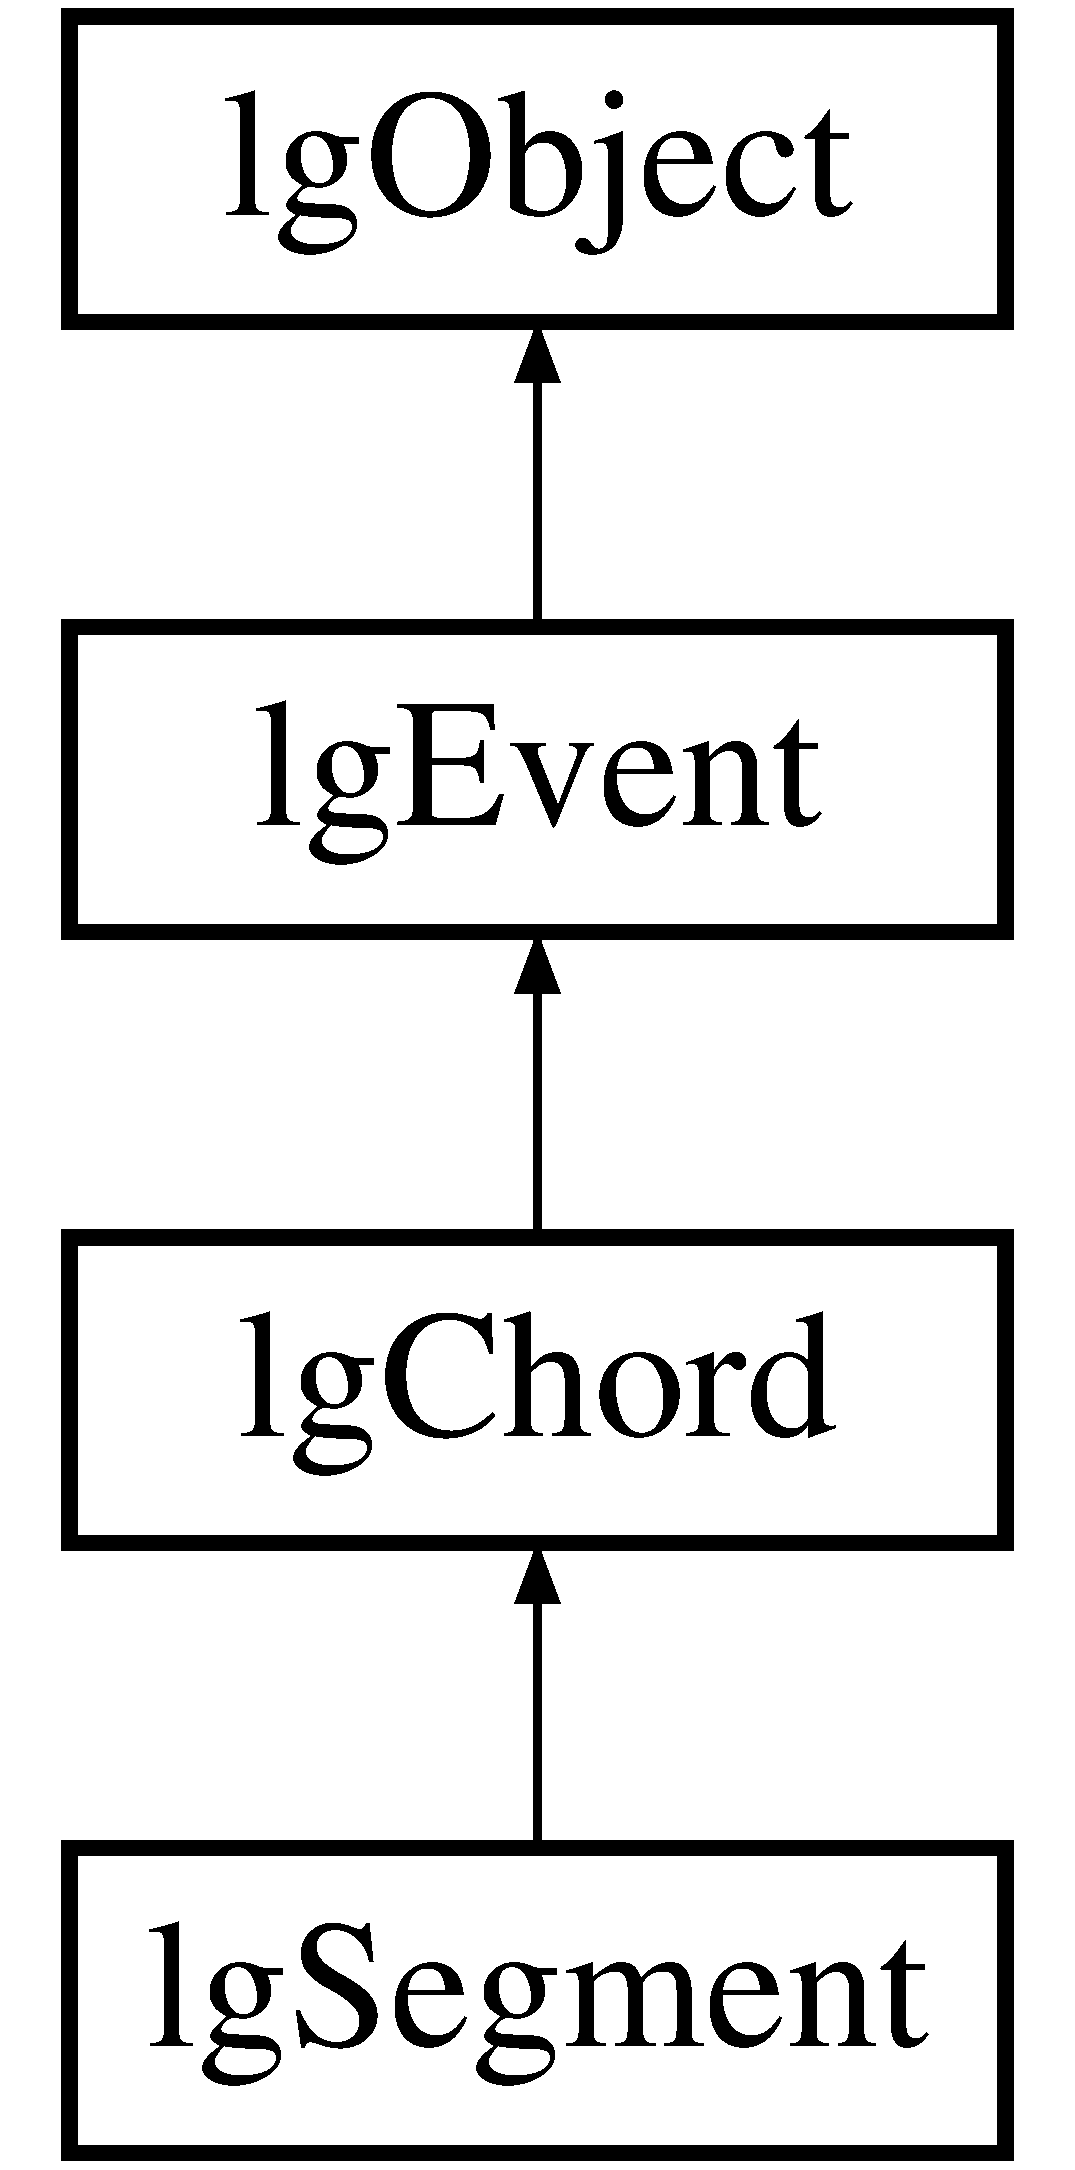
\includegraphics[height=4cm]{classlgSegment}
\end{center}
\end{figure}
\subsection*{Public Member Functions}
\begin{CompactItemize}
\item 
{\bf lg\-Segment} ({\bf lg\-Factory} $\ast$fy)
\item 
int {\bf parse\-GMNFile} (FILE $\ast$file)
\begin{CompactList}\small\item\em result: 0 == ok, 1 == parse error \item\end{CompactList}\item 
int {\bf parse\-GMNFile} (const char $\ast$filename)
\begin{CompactList}\small\item\em result: 0 == ok, 1 == parse error \item\end{CompactList}\item 
int {\bf parse\-String} (char $\ast$str)
\begin{CompactList}\small\item\em result: 0 == ok, 1 == parse error \item\end{CompactList}\item 
int {\bf parse\-String} (string str)
\begin{CompactList}\small\item\em result: 0 == ok, 1 == parse error \item\end{CompactList}\item 
virtual {\bf $\sim$lg\-Segment} (void)
\item 
virtual void {\bf append\-Event} ({\bf lg\-Event} $\ast$ev)
\begin{CompactList}\small\item\em append event in cur\-Sequence OR cur\-Chord!!! \item\end{CompactList}\item 
{\bf lg\-Rest} $\ast$ {\bf append\-Rest} (long int dur\-N, long int dur\-D, int dots, long int dur\-Pos\-N, long int dur\-Pos\-D)
\begin{CompactList}\small\item\em create a new virtual {\bf lg\-Rest} event and append \item\end{CompactList}\item 
void {\bf append\-Empty} (long int dur\-N, long int dur\-D, int dots, long int dur\-Pos\-N, long int dur\-Pos\-D)
\begin{CompactList}\small\item\em create a new virtual {\bf lg\-Empty} and append \item\end{CompactList}\item 
{\bf lg\-Note} $\ast$ {\bf append\-Note} (int pc, int oct, int acc, long int dur\-N, long int dur\-D, int dots, long int dur\-Pos\-N, long int dur\-Pos\-D)
\begin{CompactList}\small\item\em create a new virtual {\bf lg\-Note} and append \item\end{CompactList}\item 
{\bf lg\-Chord} $\ast$ {\bf append\-Chord} ({\bf lg\-Chord} $\ast$ch)
\begin{CompactList}\small\item\em append chord in cur\-Sequence, if ch == NULL -$>$ close current chord, return == appended chord! \item\end{CompactList}\item 
void {\bf insert\-Tag} ({\bf lg\-Tag} $\ast${\bf tag})
\begin{CompactList}\small\item\em append tag in cur\-Sequence \item\end{CompactList}\item 
virtual {\bf lg\-Tag} $\ast$ {\bf append\-Tag} (long int {\bf tagno}, const char $\ast$tagname)
\begin{CompactList}\small\item\em append a tag to cur\-Sequence-$>$[cur\-Chord\-Voice] \item\end{CompactList}\item 
{\bf lg\-Chord} $\ast$ {\bf init\-Chord} (long int pos\-Num, long int pos\-Denom)
\begin{CompactList}\small\item\em create a new chord in cur\-Sequence \item\end{CompactList}\item 
void {\bf init\-Chord\-Voice} (void)
\begin{CompactList}\small\item\em create a new voice in cur\-Chord \item\end{CompactList}\item 
void {\bf exit\-Chord\-Voice} (void)
\begin{CompactList}\small\item\em close cur\-Voice \item\end{CompactList}\item 
virtual {\bf lg\-Sequence} $\ast$ {\bf append\-Sequence} ({\bf lg\-Sequence} $\ast$seq=NULL)
\begin{CompactList}\small\item\em append a new sequence and store in cur\-Sequence, if seq == NULL a sequence will be created \item\end{CompactList}\item 
void {\bf exit\-Sequence} (void)
\begin{CompactList}\small\item\em leave, close the current sequence if parsing a ']' \item\end{CompactList}\item 
void {\bf close\-Tag} (long int id)
\item 
{\bf lg\-Sequence} $\ast$ {\bf first\-Sequence} (void)
\item 
{\bf lg\-Sequence} $\ast$ {\bf next\-Sequence} (void)
\item 
virtual string {\bf to\-String} ({\bf lg\-Voice} $\ast$calling\-Seq=NULL)
\begin{CompactList}\small\item\em reset the close\-Range stack for events/tags of all voices \item\end{CompactList}\item 
virtual void {\bf write} (FILE $\ast$out, {\bf lg\-Voice} $\ast$v=NULL)
\begin{CompactList}\small\item\em write own data AND all tags starting in call\-Seq in (this-$>$pos...next-$>$pos] \item\end{CompactList}\item 
virtual void {\bf write\-File} (const char $\ast$fname)
\item 
{\bf lg\-Sequence} $\ast$ {\bf search\-By\-ID} (int n)
\end{CompactItemize}
\subsection*{Public Attributes}
\begin{CompactItemize}
\item 
{\bf lg\-Factory} $\ast$ {\bf factory}
\begin{CompactList}\small\item\em ptr to the factory object \item\end{CompactList}\end{CompactItemize}
\subsection*{Private Attributes}
\begin{CompactItemize}
\item 
{\bf lg\-Sequence} $\ast$ {\bf cur\-Sequence}
\begin{CompactList}\small\item\em cur\-Pointers for parsing \item\end{CompactList}\item 
{\bf lg\-Chord} $\ast$ {\bf cur\-Chord}
\item 
{\bf lg\-Event} $\ast$ {\bf cur\-Event}
\item 
{\bf lg\-Tag} $\ast$ {\bf cur\-Tag}
\item 
{\bf lg\-Voice} $\ast$ {\bf cur\-Chord\-Voice}
\end{CompactItemize}


\subsection{Detailed Description}
GUIDO Segment based on {\bf lg\-Chord} with parsing support. 



\subsection{Constructor \& Destructor Documentation}
\index{lgSegment@{lg\-Segment}!lgSegment@{lgSegment}}
\index{lgSegment@{lgSegment}!lgSegment@{lg\-Segment}}
\subsubsection{\setlength{\rightskip}{0pt plus 5cm}lg\-Segment::lg\-Segment ({\bf lg\-Factory} $\ast$ {\em fy})}\label{classlgSegment_a0}


\index{lgSegment@{lg\-Segment}!~lgSegment@{$\sim$lgSegment}}
\index{~lgSegment@{$\sim$lgSegment}!lgSegment@{lg\-Segment}}
\subsubsection{\setlength{\rightskip}{0pt plus 5cm}lg\-Segment::$\sim${\bf lg\-Segment} (void)\hspace{0.3cm}{\tt  [virtual]}}\label{classlgSegment_a5}




\subsection{Member Function Documentation}
\index{lgSegment@{lg\-Segment}!appendChord@{appendChord}}
\index{appendChord@{appendChord}!lgSegment@{lg\-Segment}}
\subsubsection{\setlength{\rightskip}{0pt plus 5cm}{\bf lg\-Chord} $\ast$ lg\-Segment::append\-Chord ({\bf lg\-Chord} $\ast$ {\em ch})}\label{classlgSegment_a10}


append chord in cur\-Sequence, if ch == NULL -$>$ close current chord, return == appended chord! 

\index{lgSegment@{lg\-Segment}!appendEmpty@{appendEmpty}}
\index{appendEmpty@{appendEmpty}!lgSegment@{lg\-Segment}}
\subsubsection{\setlength{\rightskip}{0pt plus 5cm}void lg\-Segment::append\-Empty (long int {\em dur\-N}, long int {\em dur\-D}, int {\em dots}, long int {\em dur\-Pos\-N}, long int {\em dur\-Pos\-D})\hspace{0.3cm}{\tt  [inline]}}\label{classlgSegment_a8}


create a new virtual {\bf lg\-Empty} and append 

\index{lgSegment@{lg\-Segment}!appendEvent@{appendEvent}}
\index{appendEvent@{appendEvent}!lgSegment@{lg\-Segment}}
\subsubsection{\setlength{\rightskip}{0pt plus 5cm}void lg\-Segment::append\-Event ({\bf lg\-Event} $\ast$ {\em ev})\hspace{0.3cm}{\tt  [virtual]}}\label{classlgSegment_a6}


append event in cur\-Sequence OR cur\-Chord!!! 

we are inside a chord

create new voice in chord! 

Reimplemented from {\bf lg\-Chord} {\rm (p.\,\pageref{classlgChord_a3})}.\index{lgSegment@{lg\-Segment}!appendNote@{appendNote}}
\index{appendNote@{appendNote}!lgSegment@{lg\-Segment}}
\subsubsection{\setlength{\rightskip}{0pt plus 5cm}{\bf lg\-Note}$\ast$ lg\-Segment::append\-Note (int {\em pc}, int {\em oct}, int {\em acc}, long int {\em dur\-N}, long int {\em dur\-D}, int {\em dots}, long int {\em dur\-Pos\-N}, long int {\em dur\-Pos\-D})\hspace{0.3cm}{\tt  [inline]}}\label{classlgSegment_a9}


create a new virtual {\bf lg\-Note} and append 

\index{lgSegment@{lg\-Segment}!appendRest@{appendRest}}
\index{appendRest@{appendRest}!lgSegment@{lg\-Segment}}
\subsubsection{\setlength{\rightskip}{0pt plus 5cm}{\bf lg\-Rest}$\ast$ lg\-Segment::append\-Rest (long int {\em dur\-N}, long int {\em dur\-D}, int {\em dots}, long int {\em dur\-Pos\-N}, long int {\em dur\-Pos\-D})\hspace{0.3cm}{\tt  [inline]}}\label{classlgSegment_a7}


create a new virtual {\bf lg\-Rest} event and append 

\index{lgSegment@{lg\-Segment}!appendSequence@{appendSequence}}
\index{appendSequence@{appendSequence}!lgSegment@{lg\-Segment}}
\subsubsection{\setlength{\rightskip}{0pt plus 5cm}{\bf lg\-Sequence} $\ast$ lg\-Segment::append\-Sequence ({\bf lg\-Sequence} $\ast$ {\em seq} = NULL)\hspace{0.3cm}{\tt  [virtual]}}\label{classlgSegment_a16}


append a new sequence and store in cur\-Sequence, if seq == NULL a sequence will be created 

\index{lgSegment@{lg\-Segment}!appendTag@{appendTag}}
\index{appendTag@{appendTag}!lgSegment@{lg\-Segment}}
\subsubsection{\setlength{\rightskip}{0pt plus 5cm}{\bf lg\-Tag} $\ast$ lg\-Segment::append\-Tag (long int {\em tagno}, const char $\ast$ {\em tagname})\hspace{0.3cm}{\tt  [virtual]}}\label{classlgSegment_a12}


append a tag to cur\-Sequence-$>$[cur\-Chord\-Voice] 

create a new tag and append overwrite this function for tag semantics check! \index{lgSegment@{lg\-Segment}!closeTag@{closeTag}}
\index{closeTag@{closeTag}!lgSegment@{lg\-Segment}}
\subsubsection{\setlength{\rightskip}{0pt plus 5cm}void lg\-Segment::close\-Tag (long int {\em id})}\label{classlgSegment_a18}


\index{lgSegment@{lg\-Segment}!exitChordVoice@{exitChordVoice}}
\index{exitChordVoice@{exitChordVoice}!lgSegment@{lg\-Segment}}
\subsubsection{\setlength{\rightskip}{0pt plus 5cm}void lg\-Segment::exit\-Chord\-Voice (void)}\label{classlgSegment_a15}


close cur\-Voice 

\index{lgSegment@{lg\-Segment}!exitSequence@{exitSequence}}
\index{exitSequence@{exitSequence}!lgSegment@{lg\-Segment}}
\subsubsection{\setlength{\rightskip}{0pt plus 5cm}void lg\-Segment::exit\-Sequence (void)}\label{classlgSegment_a17}


leave, close the current sequence if parsing a ']' 

\index{lgSegment@{lg\-Segment}!firstSequence@{firstSequence}}
\index{firstSequence@{firstSequence}!lgSegment@{lg\-Segment}}
\subsubsection{\setlength{\rightskip}{0pt plus 5cm}{\bf lg\-Sequence}$\ast$ lg\-Segment::first\-Sequence (void)\hspace{0.3cm}{\tt  [inline]}}\label{classlgSegment_a19}


\index{lgSegment@{lg\-Segment}!initChord@{initChord}}
\index{initChord@{initChord}!lgSegment@{lg\-Segment}}
\subsubsection{\setlength{\rightskip}{0pt plus 5cm}{\bf lg\-Chord} $\ast$ lg\-Segment::init\-Chord (long int {\em pos\-Num}, long int {\em pos\-Denom})}\label{classlgSegment_a13}


create a new chord in cur\-Sequence 

\index{lgSegment@{lg\-Segment}!initChordVoice@{initChordVoice}}
\index{initChordVoice@{initChordVoice}!lgSegment@{lg\-Segment}}
\subsubsection{\setlength{\rightskip}{0pt plus 5cm}void lg\-Segment::init\-Chord\-Voice (void)}\label{classlgSegment_a14}


create a new voice in cur\-Chord 

\index{lgSegment@{lg\-Segment}!insertTag@{insertTag}}
\index{insertTag@{insertTag}!lgSegment@{lg\-Segment}}
\subsubsection{\setlength{\rightskip}{0pt plus 5cm}void lg\-Segment::insert\-Tag ({\bf lg\-Tag} $\ast$ {\em tag})}\label{classlgSegment_a11}


append tag in cur\-Sequence 

tag might be NULLL if it should be ignored! \index{lgSegment@{lg\-Segment}!nextSequence@{nextSequence}}
\index{nextSequence@{nextSequence}!lgSegment@{lg\-Segment}}
\subsubsection{\setlength{\rightskip}{0pt plus 5cm}{\bf lg\-Sequence}$\ast$ lg\-Segment::next\-Sequence (void)\hspace{0.3cm}{\tt  [inline]}}\label{classlgSegment_a20}


\index{lgSegment@{lg\-Segment}!parseGMNFile@{parseGMNFile}}
\index{parseGMNFile@{parseGMNFile}!lgSegment@{lg\-Segment}}
\subsubsection{\setlength{\rightskip}{0pt plus 5cm}int lg\-Segment::parse\-GMNFile (const char $\ast$ {\em filename})}\label{classlgSegment_a2}


result: 0 == ok, 1 == parse error 

parse a .gmn file and fille the data structure result: 0 = ok 1 = error

pointers for parsing \index{lgSegment@{lg\-Segment}!parseGMNFile@{parseGMNFile}}
\index{parseGMNFile@{parseGMNFile}!lgSegment@{lg\-Segment}}
\subsubsection{\setlength{\rightskip}{0pt plus 5cm}int lg\-Segment::parse\-GMNFile (FILE $\ast$ {\em file})}\label{classlgSegment_a1}


result: 0 == ok, 1 == parse error 

\index{lgSegment@{lg\-Segment}!parseString@{parseString}}
\index{parseString@{parseString}!lgSegment@{lg\-Segment}}
\subsubsection{\setlength{\rightskip}{0pt plus 5cm}int lg\-Segment::parse\-String (string {\em str})\hspace{0.3cm}{\tt  [inline]}}\label{classlgSegment_a4}


result: 0 == ok, 1 == parse error 

\index{lgSegment@{lg\-Segment}!parseString@{parseString}}
\index{parseString@{parseString}!lgSegment@{lg\-Segment}}
\subsubsection{\setlength{\rightskip}{0pt plus 5cm}int lg\-Segment::parse\-String (char $\ast$ {\em str})}\label{classlgSegment_a3}


result: 0 == ok, 1 == parse error 

\index{lgSegment@{lg\-Segment}!searchByID@{searchByID}}
\index{searchByID@{searchByID}!lgSegment@{lg\-Segment}}
\subsubsection{\setlength{\rightskip}{0pt plus 5cm}{\bf lg\-Sequence}$\ast$ lg\-Segment::search\-By\-ID (int {\em n})\hspace{0.3cm}{\tt  [inline]}}\label{classlgSegment_a24}


\index{lgSegment@{lg\-Segment}!toString@{toString}}
\index{toString@{toString}!lgSegment@{lg\-Segment}}
\subsubsection{\setlength{\rightskip}{0pt plus 5cm}virtual string lg\-Segment::to\-String ({\bf lg\-Voice} $\ast$ {\em calling\-Seq} = NULL)\hspace{0.3cm}{\tt  [inline, virtual]}}\label{classlgSegment_a21}


reset the close\-Range stack for events/tags of all voices 

write all tags between this and next call\-Seq might be NULL for Segements 

Reimplemented from {\bf lg\-Chord} {\rm (p.\,\pageref{classlgChord_a6})}.\index{lgSegment@{lg\-Segment}!write@{write}}
\index{write@{write}!lgSegment@{lg\-Segment}}
\subsubsection{\setlength{\rightskip}{0pt plus 5cm}virtual void lg\-Segment::write (FILE $\ast$ {\em out}, {\bf lg\-Voice} $\ast$ {\em v} = NULL)\hspace{0.3cm}{\tt  [inline, virtual]}}\label{classlgSegment_a22}


write own data AND all tags starting in call\-Seq in (this-$>$pos...next-$>$pos] 



Reimplemented from {\bf lg\-Chord} {\rm (p.\,\pageref{classlgChord_a7})}.\index{lgSegment@{lg\-Segment}!writeFile@{writeFile}}
\index{writeFile@{writeFile}!lgSegment@{lg\-Segment}}
\subsubsection{\setlength{\rightskip}{0pt plus 5cm}virtual void lg\-Segment::write\-File (const char $\ast$ {\em fname})\hspace{0.3cm}{\tt  [inline, virtual]}}\label{classlgSegment_a23}




\subsection{Member Data Documentation}
\index{lgSegment@{lg\-Segment}!curChord@{curChord}}
\index{curChord@{curChord}!lgSegment@{lg\-Segment}}
\subsubsection{\setlength{\rightskip}{0pt plus 5cm}{\bf lg\-Chord}$\ast$ {\bf lg\-Segment::cur\-Chord}\hspace{0.3cm}{\tt  [private]}}\label{classlgSegment_r1}


\index{lgSegment@{lg\-Segment}!curChordVoice@{curChordVoice}}
\index{curChordVoice@{curChordVoice}!lgSegment@{lg\-Segment}}
\subsubsection{\setlength{\rightskip}{0pt plus 5cm}{\bf lg\-Voice}$\ast$ {\bf lg\-Segment::cur\-Chord\-Voice}\hspace{0.3cm}{\tt  [private]}}\label{classlgSegment_r4}


\index{lgSegment@{lg\-Segment}!curEvent@{curEvent}}
\index{curEvent@{curEvent}!lgSegment@{lg\-Segment}}
\subsubsection{\setlength{\rightskip}{0pt plus 5cm}{\bf lg\-Event}$\ast$ {\bf lg\-Segment::cur\-Event}\hspace{0.3cm}{\tt  [private]}}\label{classlgSegment_r2}


\index{lgSegment@{lg\-Segment}!curSequence@{curSequence}}
\index{curSequence@{curSequence}!lgSegment@{lg\-Segment}}
\subsubsection{\setlength{\rightskip}{0pt plus 5cm}{\bf lg\-Sequence}$\ast$ {\bf lg\-Segment::cur\-Sequence}\hspace{0.3cm}{\tt  [private]}}\label{classlgSegment_r0}


cur\-Pointers for parsing 

\index{lgSegment@{lg\-Segment}!curTag@{curTag}}
\index{curTag@{curTag}!lgSegment@{lg\-Segment}}
\subsubsection{\setlength{\rightskip}{0pt plus 5cm}{\bf lg\-Tag}$\ast$ {\bf lg\-Segment::cur\-Tag}\hspace{0.3cm}{\tt  [private]}}\label{classlgSegment_r3}


\index{lgSegment@{lg\-Segment}!factory@{factory}}
\index{factory@{factory}!lgSegment@{lg\-Segment}}
\subsubsection{\setlength{\rightskip}{0pt plus 5cm}{\bf lg\-Factory}$\ast$ {\bf lg\-Segment::factory}}\label{classlgSegment_o0}


ptr to the factory object 



The documentation for this class was generated from the following files:\begin{CompactItemize}
\item 
{\bf lgsegment.h}\item 
{\bf lgsegment.cpp}\end{CompactItemize}
